
\subsection{Quinto sprint de producción}

Esta etapa contiene el desarrollo del nivel quinto del juego. El panorama general abarca un nivel de manera ascendente en un terreno nevoso. Después se llega al jefe enemigo Mictlecayotl.

Primero se empieza con el maquetado del nivel, para establecer el tamaño del nivel, nuevamente es de manera vertical el diseño, y la cámara solo se moverá en esa dirección. Se establece también donde debe ir cada objeto o enemigo junto con anotaciones necesarias para la comprensión posterior, como son direcciones de movimiento o acciones que deben realizarse. Recordando que se debe tomar muy en cuenta el tamaño del personaje a jugar si no, no se podrá avanzar en el nivel ya que se da la situación a atorarse debido al tamaño, incluido el espacio para saltar. Lo anterior se puede ver en la figura \cite{fig:n501}.
\begin{figure}[htbp]
	\centering
	\subfigure[Primera parte del nivel]{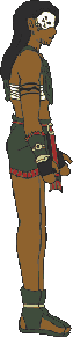
\includegraphics[width=5cm]{03TrabajoRealizado/DocProduccionR/imagenes/n5/06.png}}
	\subfigure[Segunda parte del nivel]{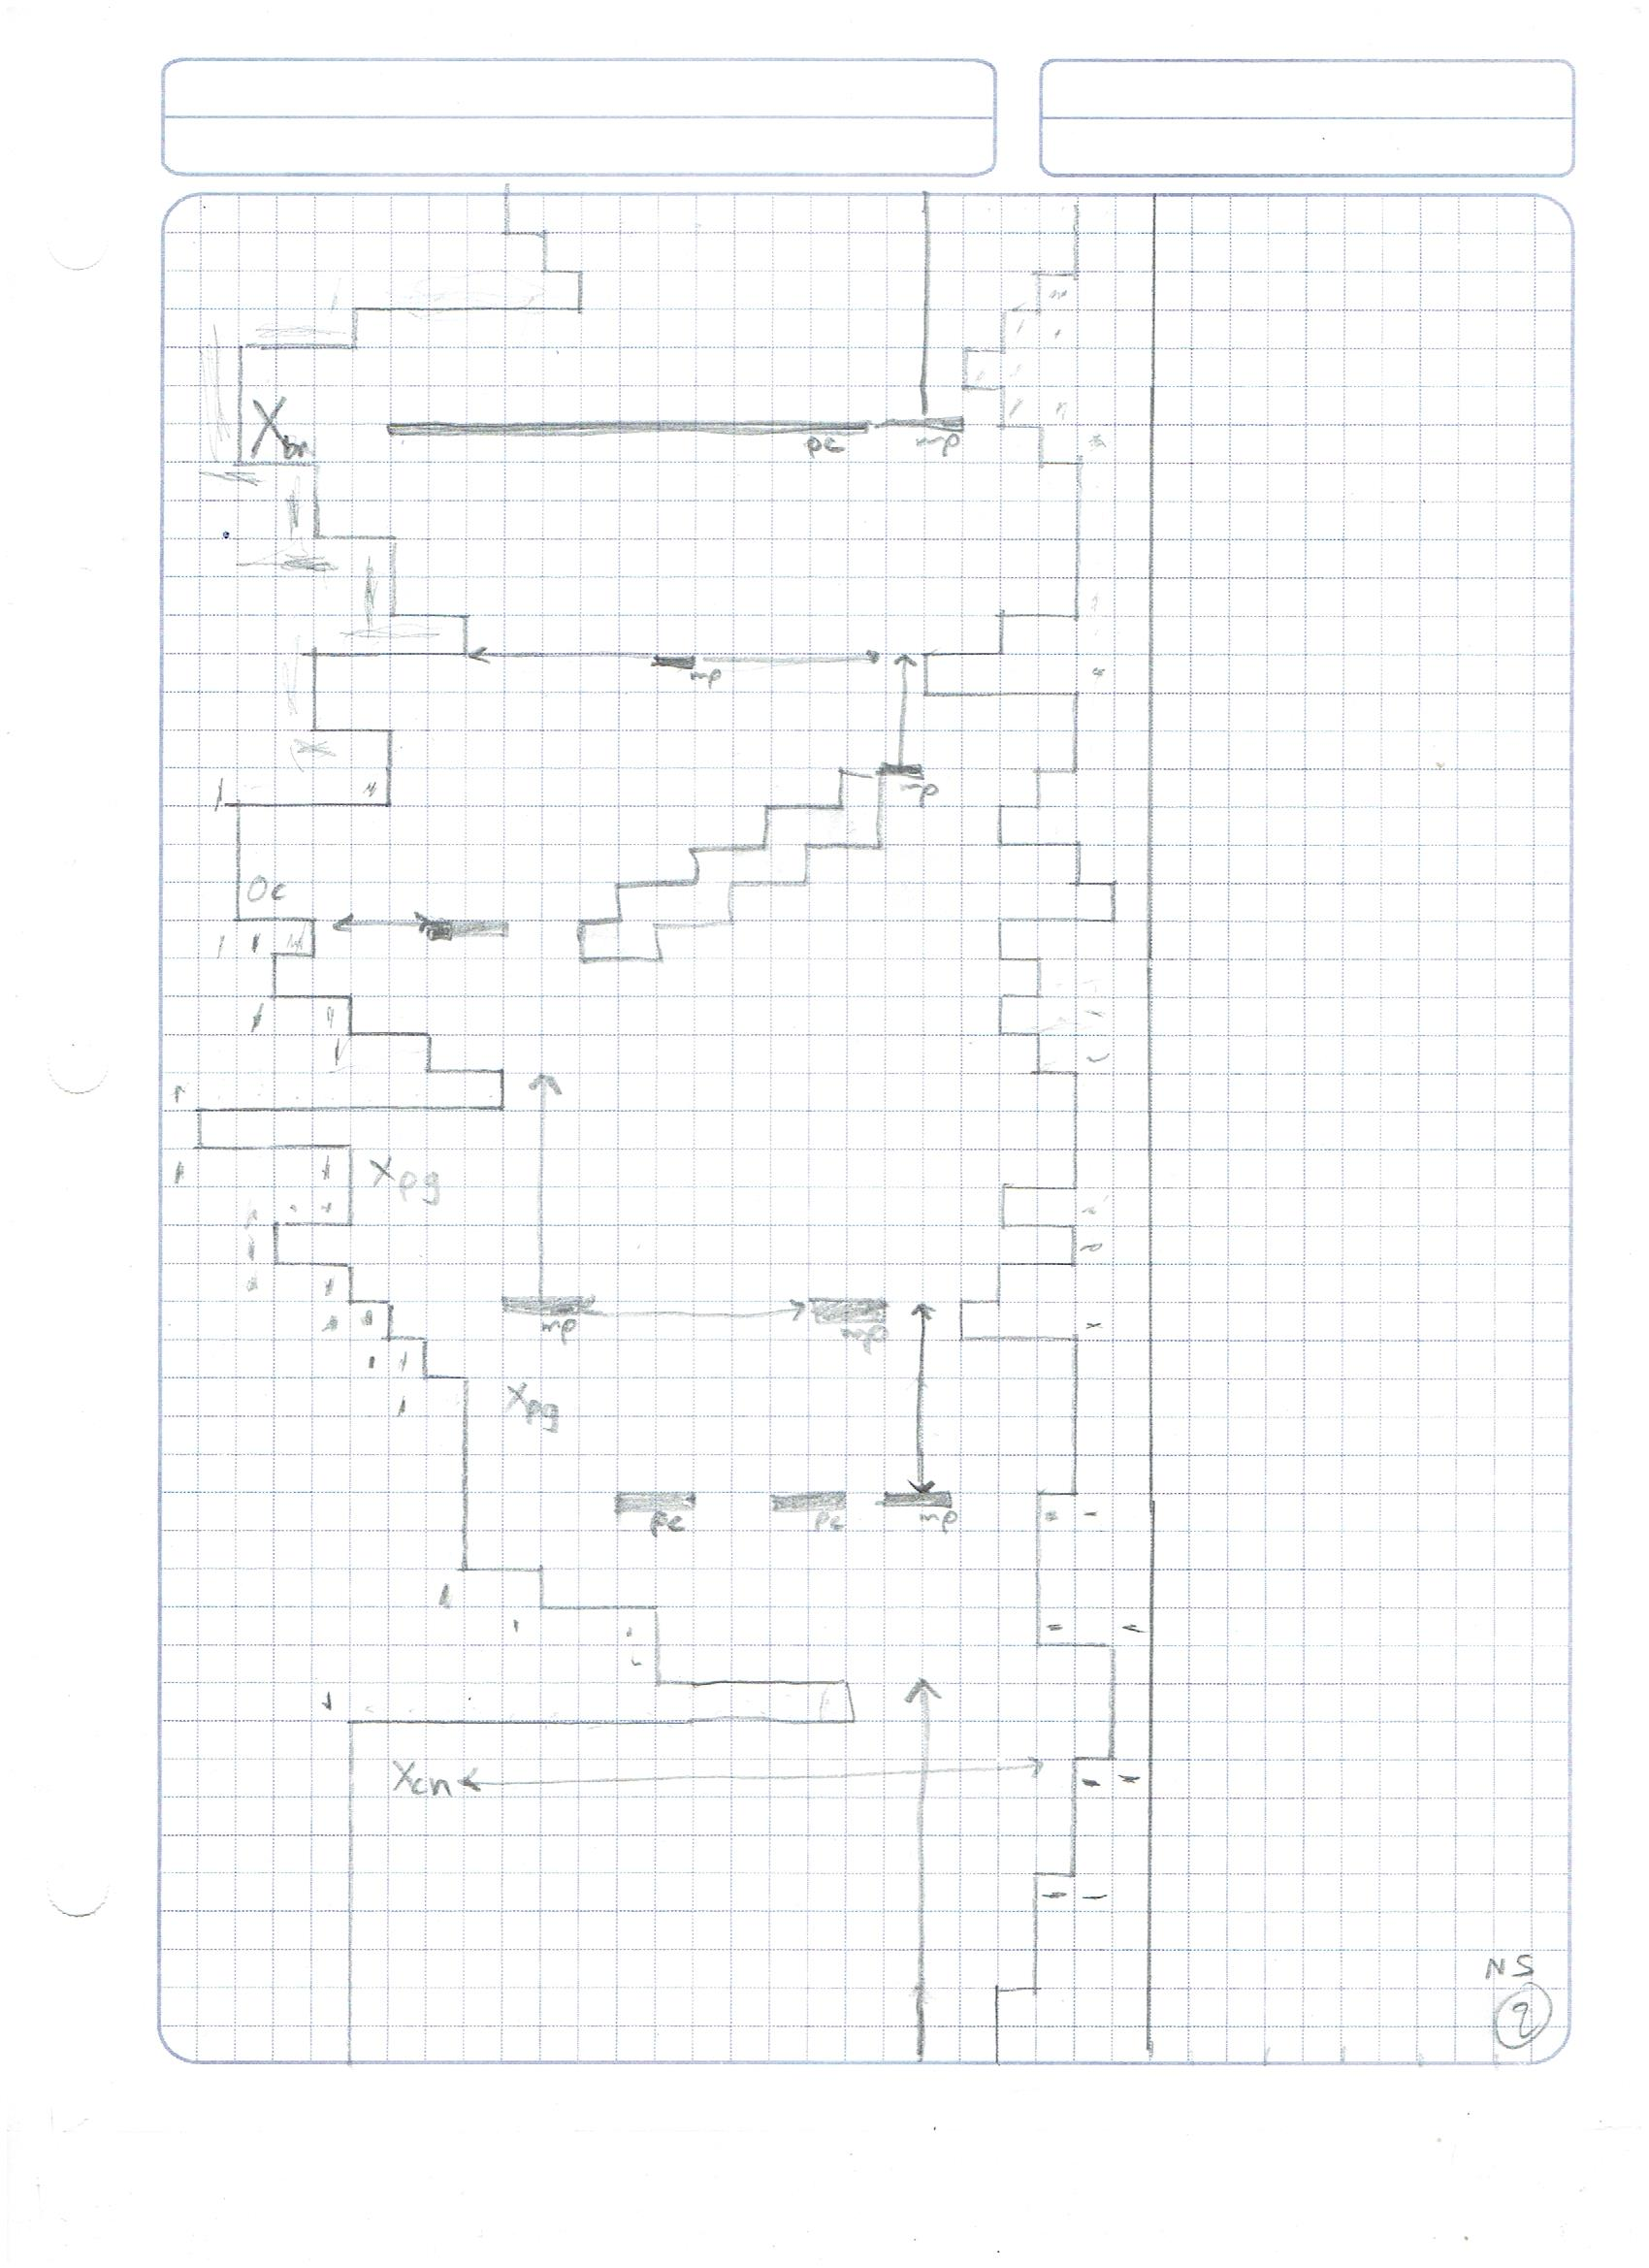
\includegraphics[width=5cm]{03TrabajoRealizado/DocProduccionR/imagenes/n5/07.png}}
	\subfigure[Tercera parte del nivel]{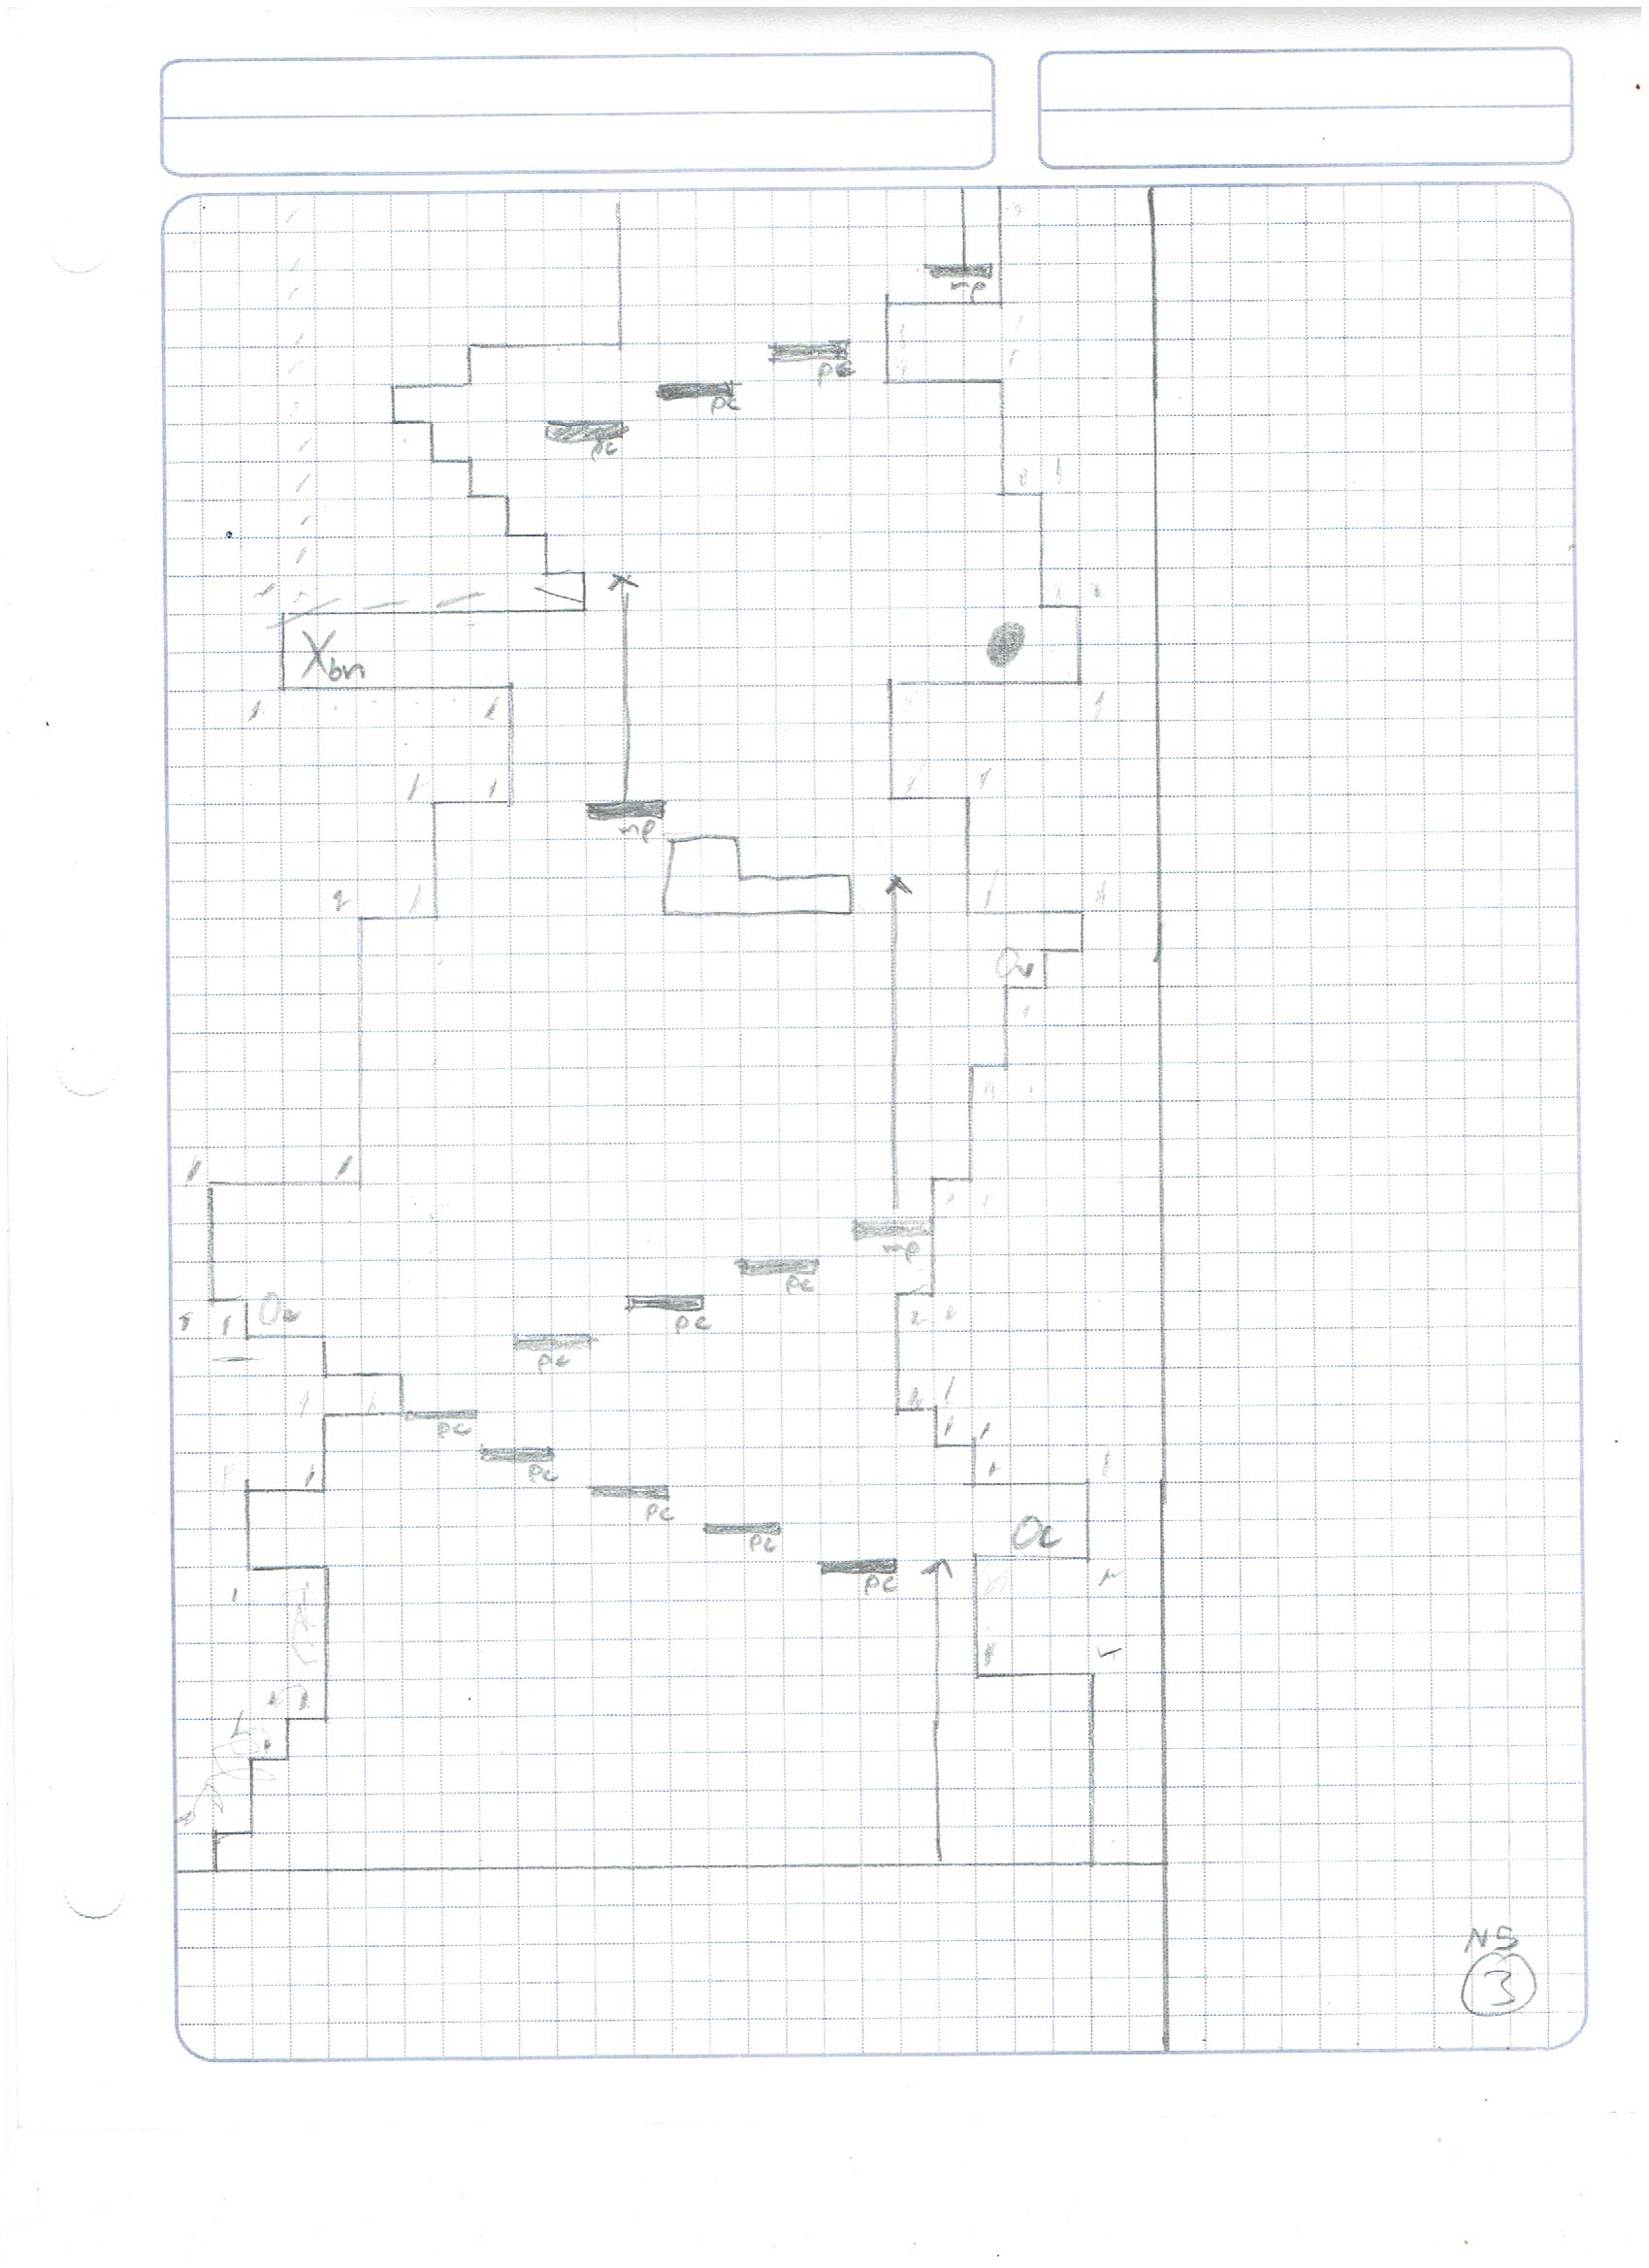
\includegraphics[width=5cm]{03TrabajoRealizado/DocProduccionR/imagenes/n5/08.png}}
	\subfigure[Cuarta parte del nivel]{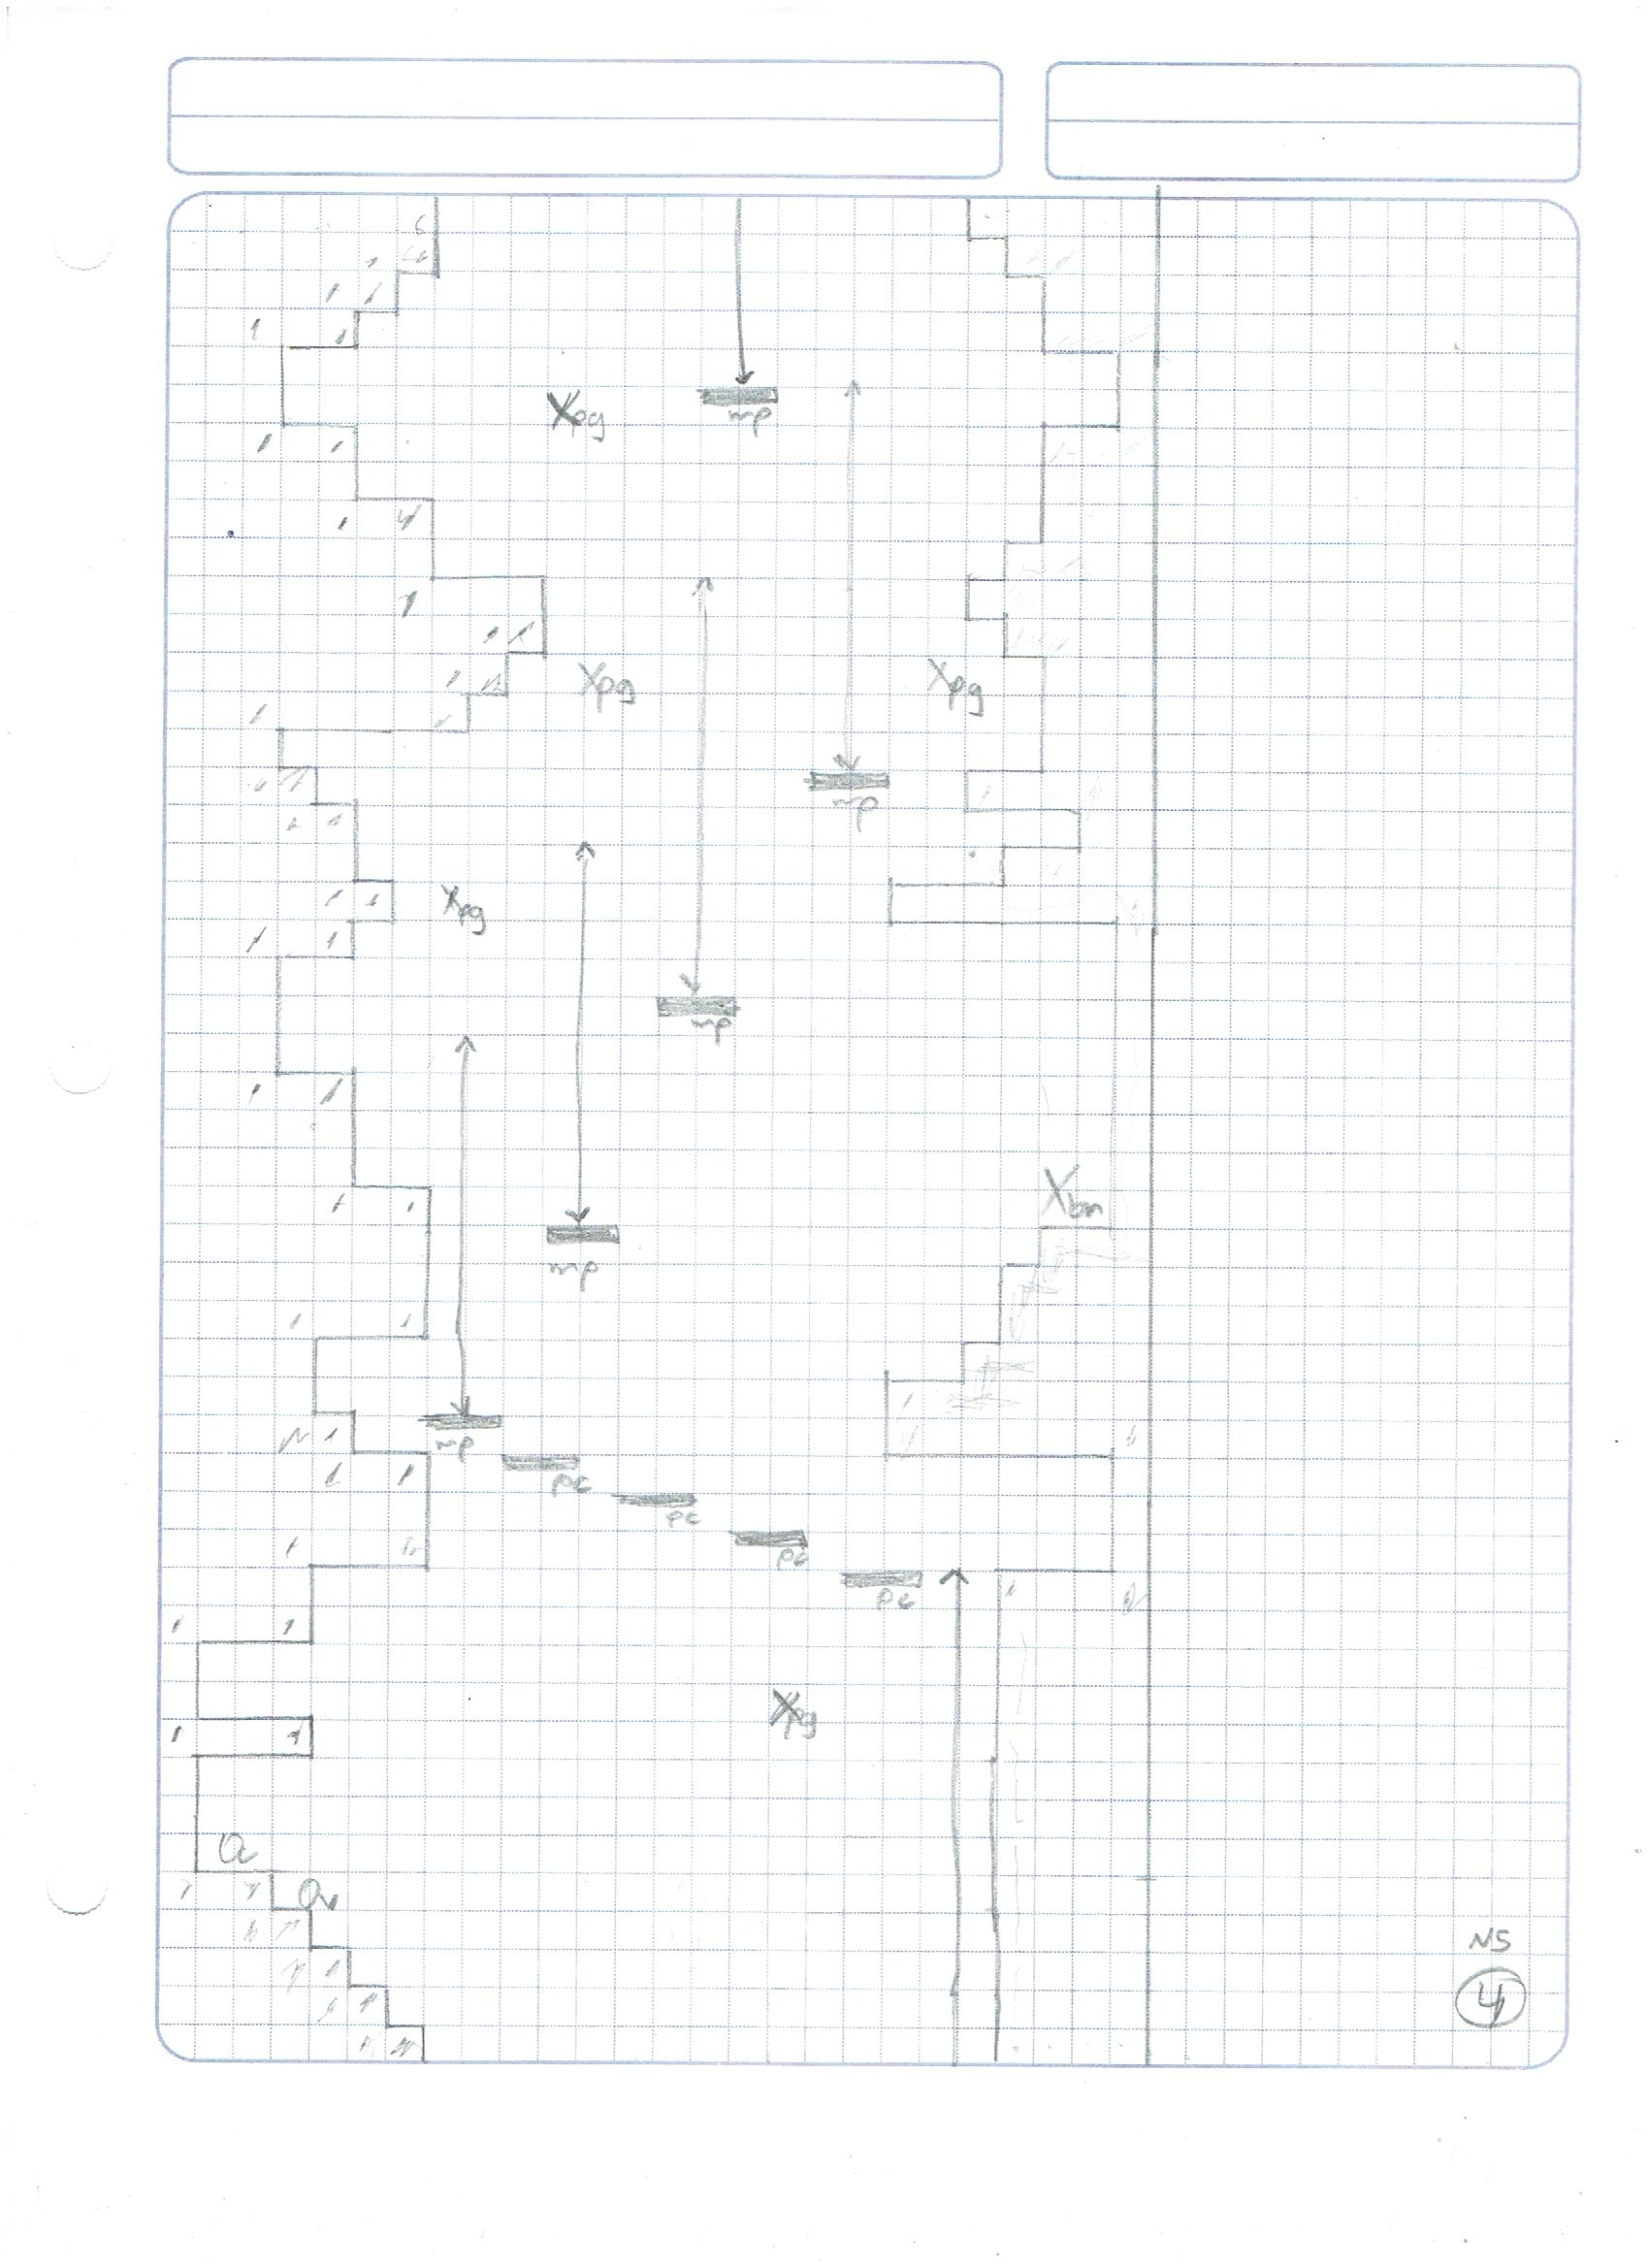
\includegraphics[width=5cm]{03TrabajoRealizado/DocProduccionR/imagenes/n5/09.png}}
	\subfigure[Quinta parte del nivel]{
\includegraphics[width=5cm]{03TrabajoRealizado/DocProduccionR/imagenes/n5/10.png}}
	\caption{Maquetado de nivel cinco} \label{fig:n501}
\end{figure}  

Después se lleva la tarea de tomar todos los componentes solo de manera visual y adecuar el tamaño necesario, tomando en cuenta las medidas de los componentes anteriores. Dichas imágenes se pueden ver en la \cite{fig:n502}.
\begin{figure}[htbp]
	\centering
	\subfigure[Imagen de viento congelante.]{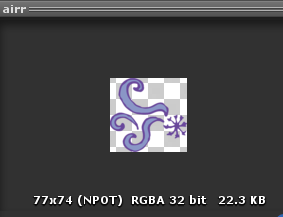
\includegraphics[width=5cm]{03TrabajoRealizado/DocProduccionR/imagenes/n5/n502.png}}
	\subfigure[Imagen de ave de nieve como enemigo.]{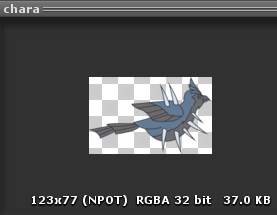
\includegraphics[width=5cm]{03TrabajoRealizado/DocProduccionR/imagenes/n5/n503.png}}
	\subfigure[Imagen de jefe enemigo Mictlecayotl]{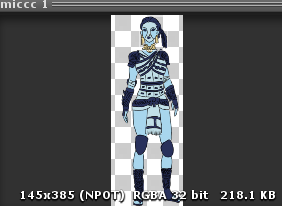
\includegraphics[width=5cm]{03TrabajoRealizado/DocProduccionR/imagenes/n5/n504.png}}
	\subfigure[Imagen de tornado.]{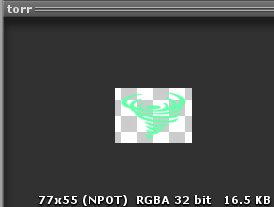
\includegraphics[width=5cm]{03TrabajoRealizado/DocProduccionR/imagenes/n5/n505.png}}
	\subfigure[Imagen de cara de jefe enemigo]{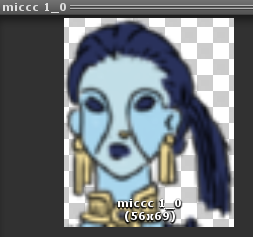
\includegraphics[width=5cm]{03TrabajoRealizado/DocProduccionR/imagenes/n5/n506.png}}
	\subfigure[Imagen de terreno.]{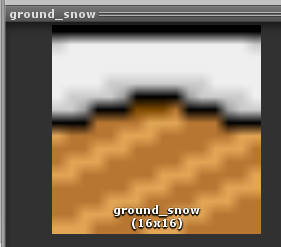
\includegraphics[width=5cm]{03TrabajoRealizado/DocProduccionR/imagenes/n5/n510.png}}
	\caption{Imágenes utilizadas para el nivel} \label{fig:n502}
\end{figure}

Después de reunir los componentes se da a la tarea de dar las acciones que realizarían descritas dentro de la figura \cite{fig:n503}. En esta parte se omite las plataformas con movimiento tanto horizontal como vertical, pues presentan el mismo comportamiento que los anteriores. También se omite los enemigos fantasmas que ya han sido realizado en los niveles anteriores.
\begin{figure}[htbp]
	\centering
	\subfigure[Detección de pase de personaje por zona determinada, donde luego la bola de nieve caerá, pero esta al final de cierto tiempo desaparecerá.]{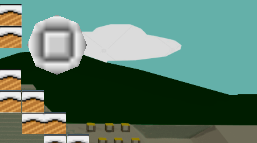
\includegraphics[width=5cm]{03TrabajoRealizado/DocProduccionR/imagenes/n5/n507.png}}
	\subfigure[Piso que desaparece despues de tocarlo simulando que se derrite, después de un tiempo establecido vuelve a aparecer.]{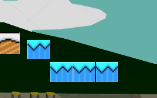
\includegraphics[width=5cm]{03TrabajoRealizado/DocProduccionR/imagenes/n5/n508.png}}
	\subfigure[Piso congelado que al ser tocado por el jugador simula que puede resbalarse sobre él.]{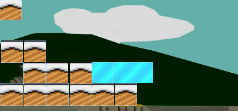
\includegraphics[width=5cm]{03TrabajoRealizado/DocProduccionR/imagenes/n5/n509.png}}
	\caption{Muestra de comportamiento de objetos} \label{fig:n503}
\end{figure}

Ya que se tiene los objetos con los comportamientos deseados se procede a ubicarlos según correspondan como se ve en la \cite{fig:n504}.
\begin{figure}
	\centering
	\caption{Maquetado llevado al motor de juego Unity.}
	\label{fig:n504}
	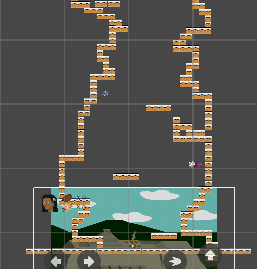
\includegraphics[width=0.5\textwidth]{03TrabajoRealizado/DocProduccionR/imagenes/n5/n501.png}
\end{figure}

Por último se establece las acciones que realiza el jefe enemigo Mictlecayotl descritas en la siguiente figura \cite{fig:n505}.
\begin{figure}[htbp]
	\centering
	\subfigure[El enemigo lanza de manera aleatoria hacia la izquierda o derecha un viento congelante.]{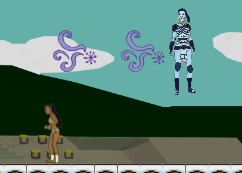
\includegraphics[width=5cm]{03TrabajoRealizado/DocProduccionR/imagenes/n5/n511.png}}
	\subfigure[El enemigo aparece de forma aleatoria por el eje horizontal sobre la superficie pequeños tornados.]{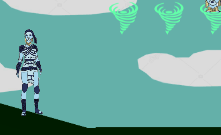
\includegraphics[width=5cm]{03TrabajoRealizado/DocProduccionR/imagenes/n5/n512.png}}
	\caption{Muestra de acciones de el jefe enemigo Mictlecayotl} \label{fig:n505}
\end{figure}